\documentclass[12pt,a4paper]{report}

% --------------------------------------------------
% Packages
% --------------------------------------------------
\usepackage{graphicx}
\usepackage{tikz}
\usetikzlibrary{arrows.meta, positioning, shapes.geometric, shapes.misc, calc}
\usepackage{float}
\usepackage{array}
\usepackage{amsmath}


% --------------------------------------------------
% Project information
% --------------------------------------------------


% --------------------------------------------------
% Self-contained title-page configuration
% --------------------------------------------------

\usepackage[a4paper,margin=1in]{geometry}
\usepackage{setspace}
\usepackage{titlesec}
\usepackage[hidelinks]{hyperref}

\newcommand{\CourseHeader}{Your Course Code - Course Title}
\newcommand{\ProjectName}{SmartCross}
\newcommand{\ProjectSubtitle}{Real-Time Railway Crossing Safety and Prediction System}
\newcommand{\StudentDetails}{%
  \texttt{1024030925} Moksh \\
  \texttt{1024030312} Sandeep Yadav \\
  \texttt{1024030314} Gagandeep Singh \\
  
}
\newcommand{\GroupDetails}{Group: \texttt{XXXX} \quad BE Third Year, CSE}
\newcommand{\AdvisorDetails}{Dr. Faculty Member Name}

% --------------------------------------------------
% TikZ diagram styles
% --------------------------------------------------
\tikzset{
  block/.style={
    rectangle,
    rounded corners,
    draw,
    align=center,
    minimum width=3.0cm,
    minimum height=0.9cm,
    inner sep=6pt,
    font=\small
  },
  actor/.style={
    rectangle,
    rounded corners,
    draw,
    align=center,
    minimum width=2.2cm,
    minimum height=0.9cm,
    inner sep=6pt,
    font=\small
  },
  decision/.style={
    diamond,
    draw,
    align=center,
    aspect=2,
    inner sep=2pt,
    font=\small
  },
  arrow/.style={-{Latex[length=2.5mm]}, thick},
  dashedarrow/.style={-{Latex[length=2.5mm]}, dashed, thick}
}

\begin{document}

% --------------------------------------------------
% Title page and contents
% --------------------------------------------------

\begin{titlepage}
\centering
\vspace*{1.5cm}

{\Large\bfseries \CourseHeader\par}
\vspace{2cm}

{\Huge\bfseries \ProjectName\par}
\vspace{0.7cm}

{\Large \ProjectSubtitle\par}
\vspace{2cm}

{\large
\StudentDetails\par}
\vspace{1.2cm}

{\large \GroupDetails\par}
\vspace{1.2cm}

{\large\bfseries Faculty Advisor\par}
{\large \AdvisorDetails\par}

\vfill

{\large\bfseries Mid-Semester Evaluation\par}
\vspace{0.3cm}
{\large Computer Science and Engineering Department\par}
{\large Thapar Institute of Engineering and Technology, Patiala\par}

\end{titlepage}
\tableofcontents

% ==================================================
% CHAPTER 1
% ==================================================

\chapter{Introduction}

\section{Background and Context}

Railway level crossings are locations where road users and railway traffic share the
same point of intersection. At an unmanned or busy crossing, a user may not know
when a train is approaching, how long the crossing is expected to remain closed, or
whether it is safe to proceed.

SmartCross is proposed as a real-time railway crossing information and safety
system. It combines live train information with railway-crossing information to
estimate the arrival of a train at a crossing and provide useful status information
to the user.

The objective is not merely to display the location of a train. SmartCross processes
live train information and converts it into a user-oriented prediction such as
whether a crossing is open, likely to close soon, currently closed, or likely to
open soon.

\section{Problem Statement}

A road user approaching a railway crossing generally has limited information about
the current or expected state of the crossing. Existing train-tracking systems may
provide train location but do not necessarily answer the more practical question:
``What is going to happen at the crossing I am approaching?''

SmartCross addresses this problem by connecting live train information with
crossing-specific logic and presenting the resulting prediction through a web
application.

\section{Project Objectives}

\begin{enumerate}
  \item Develop a system that receives live train information from an external
        railway data source.
  \item Map relevant train movement to railway crossings and estimate the expected
        arrival time of a train at the crossing.
  \item Predict and display the crossing state, including open, closing soon,
        closed, and opening soon.
  \item Provide estimated waiting information so that users can make safer travel
        decisions.
  \item Build a scalable backend using Node.js, Express, and MongoDB with a
        web-based user interface.
\end{enumerate}

% ==================================================
% CHAPTER 2
% ==================================================

\chapter{Methodology and Design}

\section{System Architecture}

SmartCross follows a client-server architecture. The backend receives live train
data, processes the train's position and movement, calculates an estimated time
to the relevant railway crossing, and generates a crossing-status prediction.
The frontend presents this information to the user.

\subsection{High-Level Design}

Figure~\ref{fig:architecture} shows the major components of the SmartCross system.

\begin{figure}[H]
\centering
\resizebox{\textwidth}{!}{%
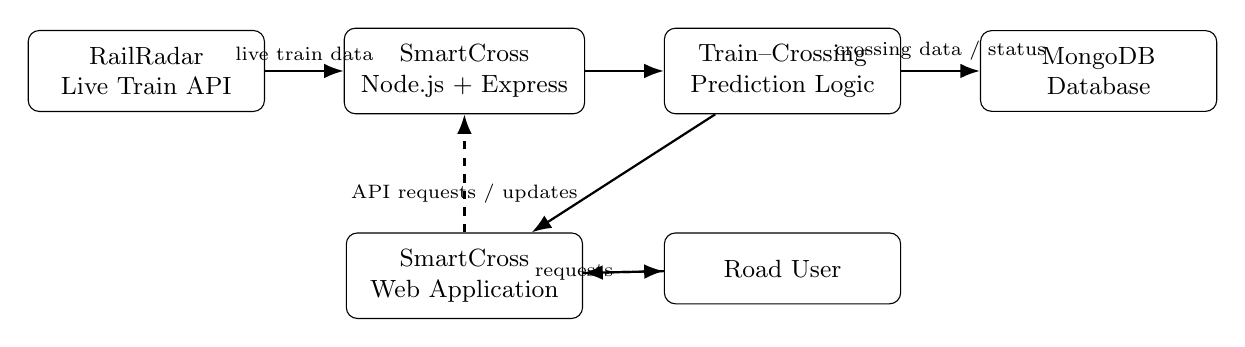
\begin{tikzpicture}[node distance=1.3cm and 1.0cm]
  \node[block] (api) {RailRadar\\Live Train API};
  \node[block, right=of api] (backend) {SmartCross\\Node.js + Express};
  \node[block, right=of backend] (logic) {Train--Crossing\\Prediction Logic};
  \node[block, right=of logic] (db) {MongoDB\\Database};

  \node[block, below=1.5cm of backend] (frontend) {SmartCross\\Web Application};
  \node[block, below=1.5cm of logic] (user) {Road User};

  \draw[arrow] (api) -- node[above,font=\scriptsize]{live train data} (backend);
  \draw[arrow] (backend) -- (logic);
  \draw[arrow] (logic) -- node[above,font=\scriptsize]{crossing data / status} (db);
  \draw[arrow] (logic) -- (frontend);
  \draw[arrow] (frontend) -- (user);
  \draw[dashedarrow] (user) -- node[left,font=\scriptsize]{requests} (frontend);
  \draw[dashedarrow] (frontend) -- node[below,font=\scriptsize]{API requests / updates} (backend);
\end{tikzpicture}%
}
\caption{High-Level SmartCross System Architecture}
\label{fig:architecture}
\end{figure}

\subsection{Technical Stack}

\begin{itemize}
  \item \textbf{Backend:} Node.js and Express.js.
  \item \textbf{Database:} MongoDB.
  \item \textbf{External Data Source:} RailRadar live train API.
  \item \textbf{Frontend:} Web-based React application.
  \item \textbf{Real-Time Communication:} WebSocket/Socket.IO can be used for
        pushing updated status to connected clients.
  \item \textbf{Development and Testing:} REST API testing tools and local
        development environment.
\end{itemize}

\section{Implementation Details}

\subsection{Live Train Data Module}

The live train data module obtains information about the relevant train from the
external railway API. The backend validates and processes the received information
before using it for crossing prediction.

A mock-data mode can also be maintained during development so that the application
can be tested when live API access is unavailable.

\subsection{Train--Crossing Prediction Module}

The prediction module determines the expected time at which a train will affect a
particular crossing. A simplified estimation can be represented as:

\[
T_{\mathrm{arrival}} =
\frac{D_{\mathrm{crossing}}}{V_{\mathrm{train}}}
\]

where $D_{\mathrm{crossing}}$ is the relevant distance between the train and the
crossing and $V_{\mathrm{train}}$ is the estimated train speed.

The system can then compare the estimated arrival time with configured crossing
timings to determine an appropriate user-facing state.

\subsection{Crossing Status Module}

The crossing-status module converts the prediction into understandable states:

\begin{itemize}
  \item \textbf{Open:} No immediate train-related closure is expected.
  \item \textbf{Closing Soon:} A relevant train is expected to reach the crossing
        soon.
  \item \textbf{Closed:} The crossing is expected to be unavailable because of the
        train.
  \item \textbf{Opening Soon:} The train has passed or is sufficiently clear and
        the crossing is expected to become available.
\end{itemize}

\subsection{User Notification Module}

The frontend presents the crossing state, expected train information, and estimated
waiting time. This allows a road user to decide whether to wait or consider an
alternative route.

% ==================================================
% CHAPTER 3 - REQUIREMENTS AND UML
% ==================================================

\chapter{Requirements and UML Design}

\section{Functional Requirements}

\begin{enumerate}
  \item The system shall obtain live train information.
  \item The system shall identify the relevant railway crossing for a train.
  \item The system shall estimate train arrival time at the crossing.
  \item The system shall determine a predicted crossing status.
  \item The system shall display crossing status to the user.
  \item The system shall display relevant train and waiting-time information.
  \item The system shall store required crossing and system data in MongoDB.
\end{enumerate}

\section{Non-Functional Requirements}

\begin{itemize}
  \item \textbf{Availability:} The system should continue to provide useful
        information whenever valid train data is available.
  \item \textbf{Performance:} API responses and status updates should be generated
        quickly enough for real-time use.
  \item \textbf{Scalability:} The backend should support multiple crossings and
        multiple users.
  \item \textbf{Usability:} Crossing status should be easy to understand at a
        glance.
  \item \textbf{Reliability:} Invalid or unavailable external data should be
        handled gracefully.
\end{itemize}

% --------------------------------------------------
% Use Case Diagram
% --------------------------------------------------

\section{Use Case Diagram}

The use case diagram identifies the major interactions between SmartCross users
and the system.

\begin{figure}[H]
\centering
\resizebox{0.95\textwidth}{!}{%
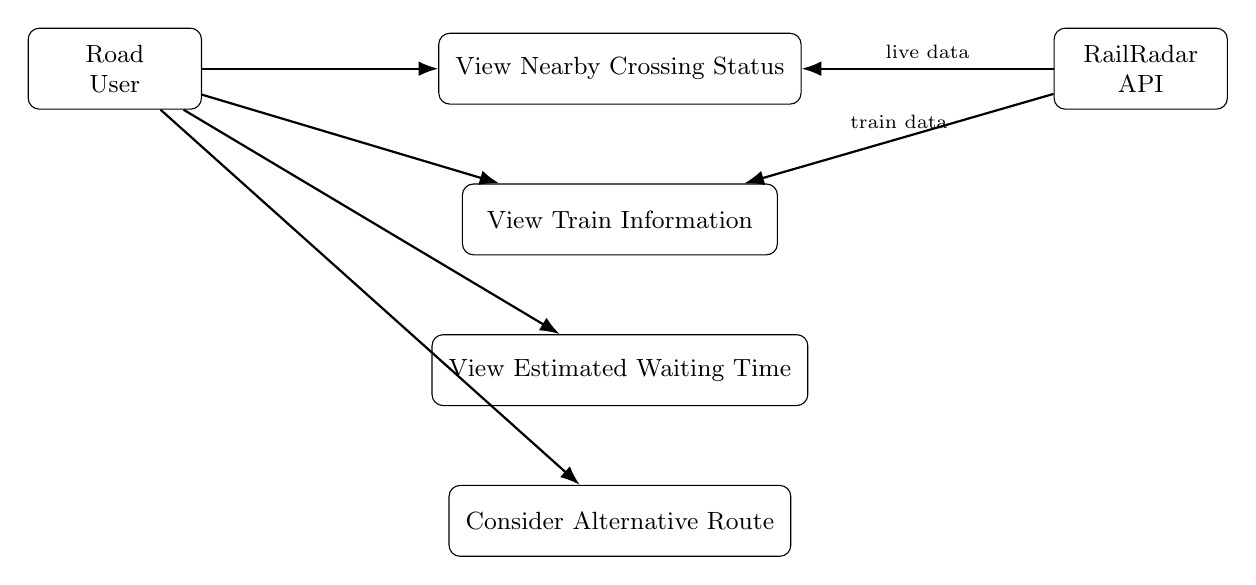
\begin{tikzpicture}[node distance=1.0cm and 1.6cm]
  \node[actor] (user) {Road\\User};

  \node[block, right=3.0cm of user, minimum width=4.0cm] (view)
        {View Nearby Crossing Status};
  \node[block, below=of view, minimum width=4.0cm] (train)
        {View Train Information};
  \node[block, below=of train, minimum width=4.0cm] (wait)
        {View Estimated Waiting Time};
  \node[block, below=of wait, minimum width=4.0cm] (route)
        {Consider Alternative Route};

  \draw[arrow] (user) -- (view);
  \draw[arrow] (user) -- (train);
  \draw[arrow] (user) -- (wait);
  \draw[arrow] (user) -- (route);

  \node[actor, right=3.2cm of view] (api)
        {RailRadar\\API};

  \draw[arrow] (api) -- node[above,font=\scriptsize]{live data} (view);
  \draw[arrow] (api) -- node[above,font=\scriptsize]{train data} (train);
\end{tikzpicture}%
}
\caption{SmartCross Use Case Diagram}
\label{fig:usecase}
\end{figure}

\section{UML Component Diagram}

The following UML-oriented component view shows how the principal software
components communicate.

\begin{figure}[H]
\centering
\resizebox{\textwidth}{!}{%
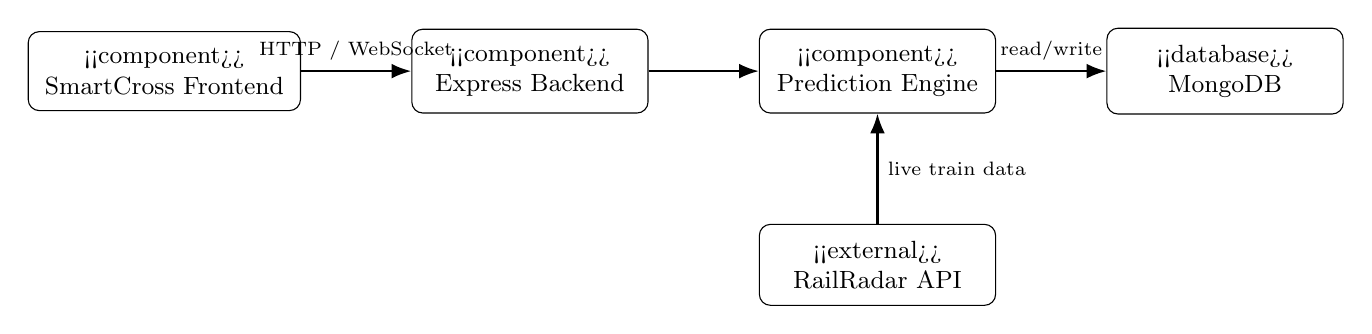
\begin{tikzpicture}[node distance=1.4cm and 1.4cm]
  \node[block] (client) {<<component>>\\SmartCross Frontend};
  \node[block, right=of client] (server) {<<component>>\\Express Backend};
  \node[block, right=of server] (predict) {<<component>>\\Prediction Engine};
  \node[block, right=of predict] (database) {<<database>>\\MongoDB};
  \node[block, below=1.4cm of predict] (rail) {<<external>>\\RailRadar API};

  \draw[arrow] (client) -- node[above,font=\scriptsize]{HTTP / WebSocket} (server);
  \draw[arrow] (server) -- (predict);
  \draw[arrow] (predict) -- node[above,font=\scriptsize]{read/write} (database);
  \draw[arrow] (rail) -- node[right,font=\scriptsize]{live train data} (predict);
\end{tikzpicture}%
}
\caption{UML Component View of SmartCross}
\label{fig:umlcomponent}
\end{figure}

% --------------------------------------------------
% Activity Diagram
% --------------------------------------------------

\section{Activity Diagram}

The activity diagram describes the flow from receiving live train data to showing
the crossing status to a road user.

\begin{figure}[H]
\centering
\resizebox{0.72\textwidth}{!}{%
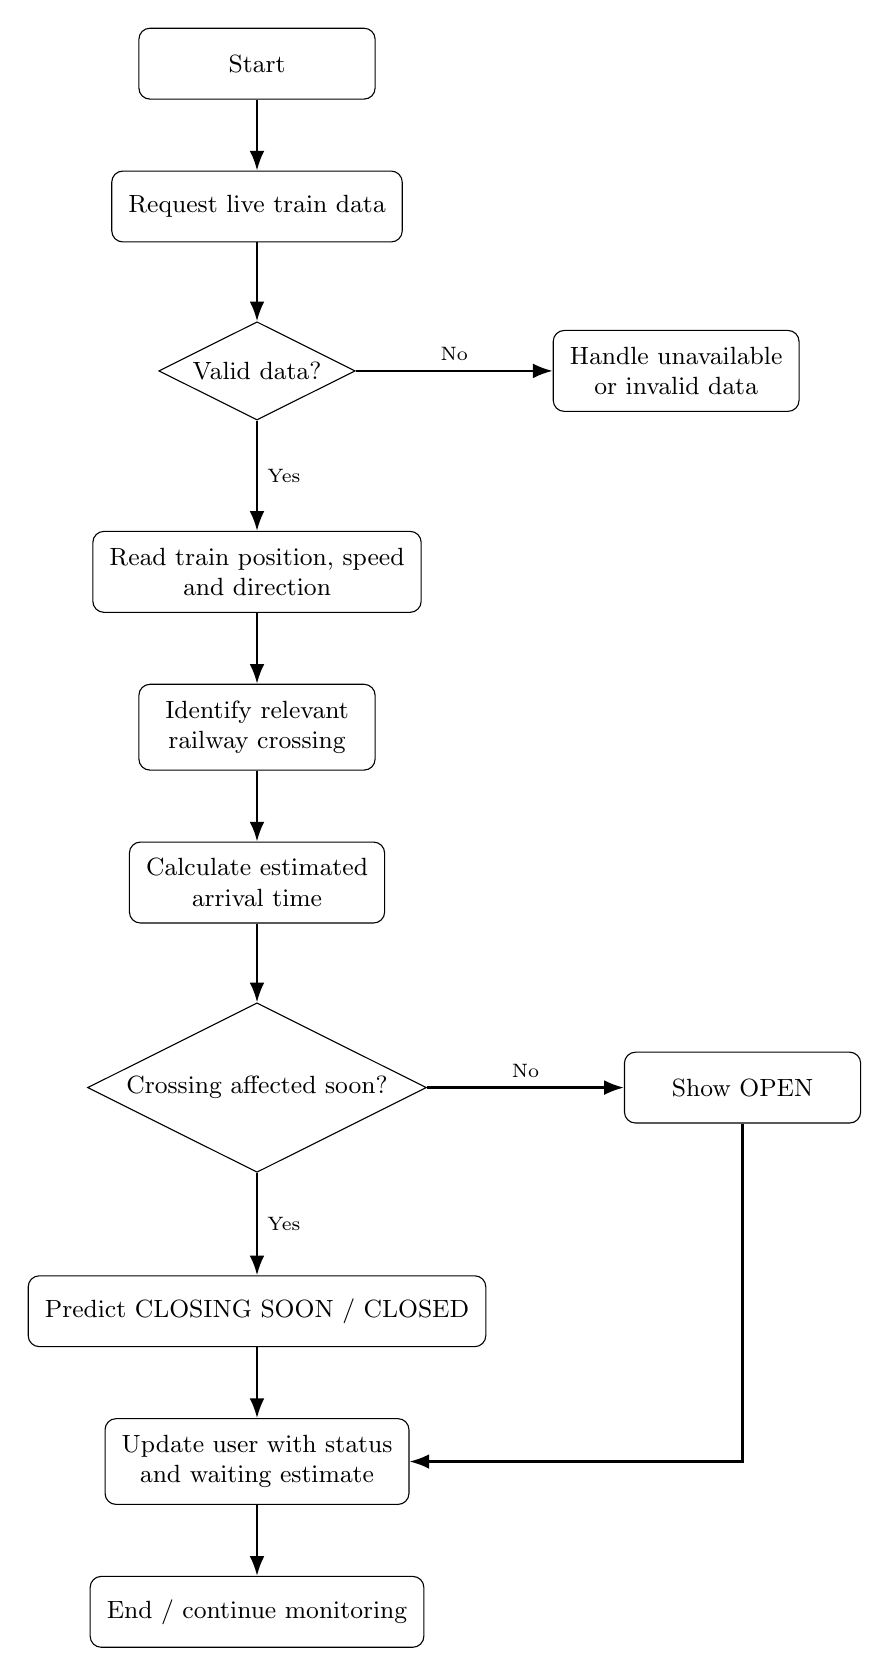
\begin{tikzpicture}[node distance=0.9cm]
  \node[block] (start) {Start};
  \node[block, below=of start] (request) {Request live train data};
  \node[decision, below=1.0cm of request] (valid) {Valid data?};

  \node[block, right=2.5cm of valid] (retry)
        {Handle unavailable\\or invalid data};
  \node[block, below=1.4cm of valid] (loc)
        {Read train position, speed\\and direction};
  \node[block, below=of loc] (cross)
        {Identify relevant\\railway crossing};
  \node[block, below=of cross] (eta)
        {Calculate estimated\\arrival time};
  \node[decision, below=1.0cm of eta] (status)
        {Crossing affected soon?};

  \node[block, right=2.5cm of status] (open)
        {Show OPEN};
  \node[block, below=1.3cm of status] (close)
        {Predict CLOSING SOON / CLOSED};
  \node[block, below=of close] (update)
        {Update user with status\\and waiting estimate};
  \node[block, below=of update] (end)
        {End / continue monitoring};

  \draw[arrow] (start) -- (request);
  \draw[arrow] (request) -- (valid);
  \draw[arrow] (valid) -- node[above,font=\scriptsize]{No} (retry);
  \draw[arrow] (valid) -- node[right,font=\scriptsize]{Yes} (loc);
  \draw[arrow] (loc) -- (cross);
  \draw[arrow] (cross) -- (eta);
  \draw[arrow] (eta) -- (status);
  \draw[arrow] (status) -- node[above,font=\scriptsize]{No} (open);
  \draw[arrow] (status) -- node[right,font=\scriptsize]{Yes} (close);
  \draw[arrow] (close) -- (update);
  \draw[arrow] (open) |- (update);
  \draw[arrow] (update) -- (end);
\end{tikzpicture}%
}
\caption{SmartCross Activity Diagram}
\label{fig:activity}
\end{figure}

% --------------------------------------------------
% Class Diagram
% --------------------------------------------------

\section{Class Diagram}

The class diagram presents the principal entities used by the SmartCross
application. The exact implementation classes may be refined during development.

\begin{figure}[H]
\centering
\resizebox{0.95\textwidth}{!}{%
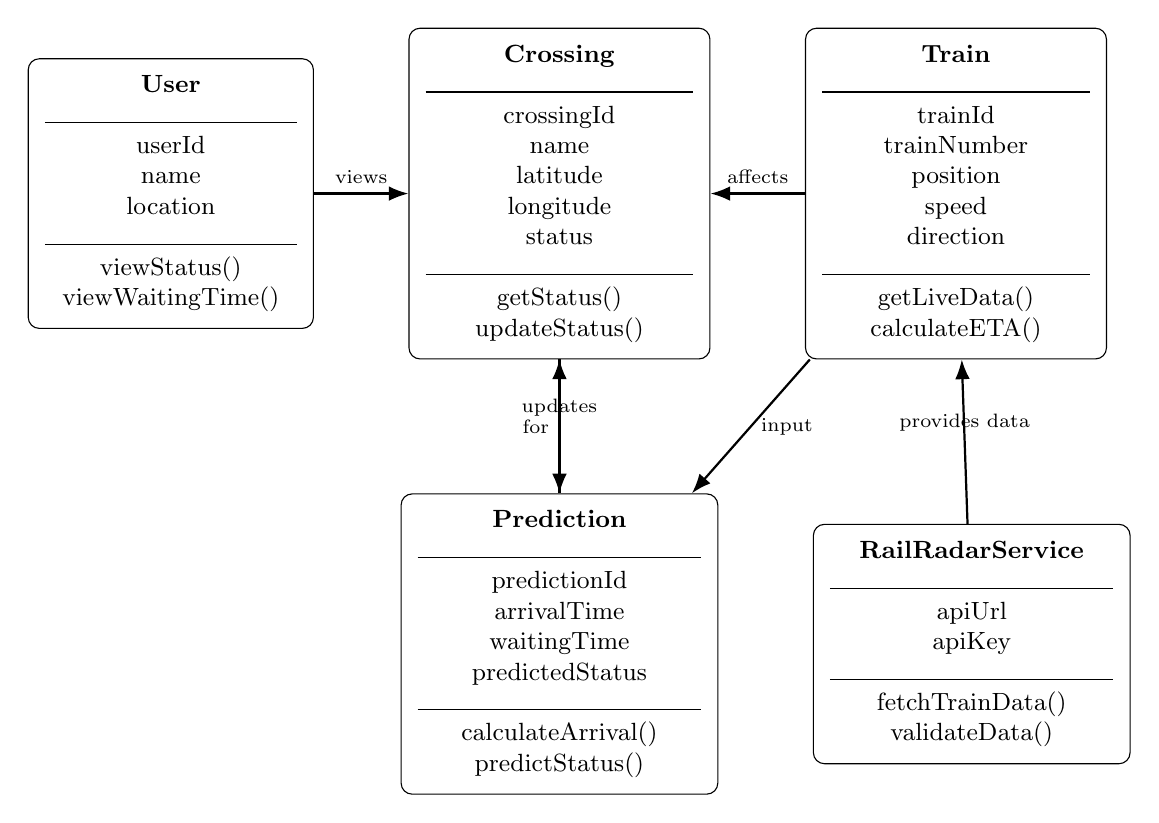
\begin{tikzpicture}[node distance=1.8cm and 1.2cm]
  \node[block, minimum width=3.6cm, minimum height=2.7cm] (user)
  {\textbf{User}\\
   \rule{3.2cm}{0.4pt}\\
   userId\\
   name\\
   location\\
   \rule{3.2cm}{0.4pt}\\
   viewStatus()\\
   viewWaitingTime()};

  \node[block, right=of user, minimum width=3.8cm, minimum height=3.0cm] (cross)
  {\textbf{Crossing}\\
   \rule{3.4cm}{0.4pt}\\
   crossingId\\
   name\\
   latitude\\
   longitude\\
   status\\
   \rule{3.4cm}{0.4pt}\\
   getStatus()\\
   updateStatus()};

  \node[block, right=of cross, minimum width=3.8cm, minimum height=3.0cm] (train)
  {\textbf{Train}\\
   \rule{3.4cm}{0.4pt}\\
   trainId\\
   trainNumber\\
   position\\
   speed\\
   direction\\
   \rule{3.4cm}{0.4pt}\\
   getLiveData()\\
   calculateETA()};

  \node[block, below=1.7cm of cross, minimum width=4.0cm, minimum height=3.0cm] (prediction)
  {\textbf{Prediction}\\
   \rule{3.6cm}{0.4pt}\\
   predictionId\\
   arrivalTime\\
   waitingTime\\
   predictedStatus\\
   \rule{3.6cm}{0.4pt}\\
   calculateArrival()\\
   predictStatus()};

  \node[block, right=of prediction, minimum width=4.0cm, minimum height=3.0cm] (api)
  {\textbf{RailRadarService}\\
   \rule{3.6cm}{0.4pt}\\
   apiUrl\\
   apiKey\\
   \rule{3.6cm}{0.4pt}\\
   fetchTrainData()\\
   validateData()};

  \draw[arrow] (user) -- node[above,font=\scriptsize]{views} (cross);
  \draw[arrow] (train) -- node[above,font=\scriptsize]{affects} (cross);
  \draw[arrow] (train) -- node[right,font=\scriptsize]{input} (prediction);
  \draw[arrow] (cross) -- node[left,font=\scriptsize]{for} (prediction);
  \draw[arrow] (api) -- node[above,font=\scriptsize]{provides data} (train);
  \draw[arrow] (prediction) -- node[above,font=\scriptsize]{updates} (cross);
\end{tikzpicture}%
}
\caption{SmartCross Class Diagram}
\label{fig:class}
\end{figure}

% --------------------------------------------------
% SDLC Diagram
% --------------------------------------------------

\section{SDLC Diagram}

SmartCross follows an iterative Software Development Life Cycle (SDLC). Each
stage produces inputs for the next stage and feedback can be used to improve
earlier stages.

\begin{figure}[H]
\centering
\resizebox{0.95\textwidth}{!}{%
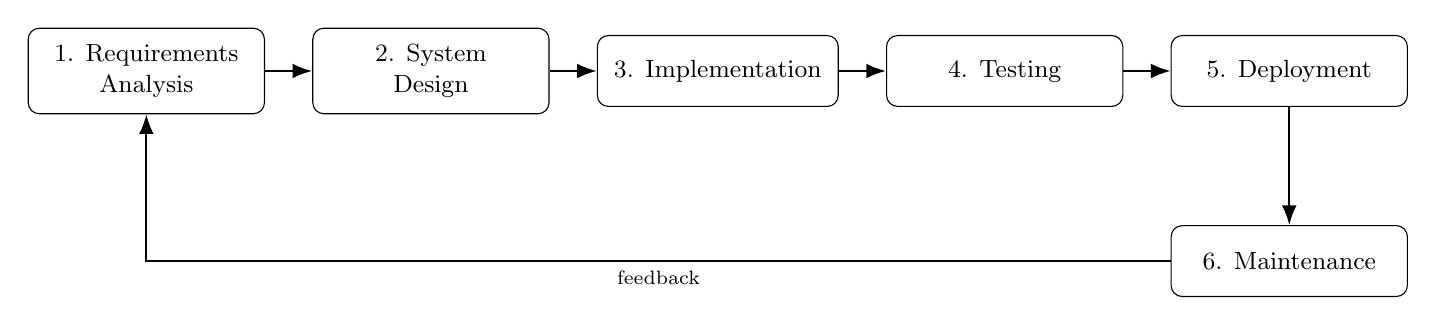
\begin{tikzpicture}[node distance=1.3cm and 0.6cm]
  \node[block] (req) {1. Requirements\\Analysis};
  \node[block, right=of req] (design) {2. System\\Design};
  \node[block, right=of design] (impl) {3. Implementation};
  \node[block, right=of impl] (test) {4. Testing};
  \node[block, right=of test] (deploy) {5. Deployment};
  \node[block, below=1.5cm of deploy] (maint) {6. Maintenance};

  \draw[arrow] (req) -- (design);
  \draw[arrow] (design) -- (impl);
  \draw[arrow] (impl) -- (test);
  \draw[arrow] (test) -- (deploy);
  \draw[arrow] (deploy) -- (maint);
  \draw[arrow] (maint) -| node[pos=0.25,below,font=\scriptsize]{feedback} (req);
\end{tikzpicture}%
}
\caption{SDLC Model Used for SmartCross}
\label{fig:sdlc}
\end{figure}

\subsection{SDLC Stages}

\begin{enumerate}
  \item \textbf{Requirements Analysis:} Identify the railway-crossing safety
        problem and define system requirements.
  \item \textbf{System Design:} Design the frontend, backend, database,
        prediction logic, APIs, and UML models.
  \item \textbf{Implementation:} Develop the Node.js/Express backend, MongoDB
        models, frontend, API integration, and prediction logic.
  \item \textbf{Testing:} Perform unit, integration, API, and user-interface
        testing.
  \item \textbf{Deployment:} Deploy the web application and configure the
        production environment.
  \item \textbf{Maintenance:} Monitor the system, handle API changes, fix bugs,
        and improve prediction and user experience.
\end{enumerate}

% ==================================================
% CHAPTER 4
% ==================================================

\chapter{Results and Evaluation}

\section{Testing Methodology}

The SmartCross system can be evaluated using the following testing levels:

\begin{itemize}
  \item \textbf{Unit Testing:} Test individual prediction, validation, and
        database functions.
  \item \textbf{Integration Testing:} Verify that the frontend, backend,
        database, and external train API work together.
  \item \textbf{API Testing:} Test live and mock train-data responses and verify
        handling of invalid or unavailable responses.
  \item \textbf{Performance Testing:} Measure response time and behaviour under
        multiple requests.
  \item \textbf{User Testing:} Verify that crossing status and waiting information
        are understandable to users.
\end{itemize}

\section{Performance Metrics}

Actual measured values should be inserted after testing. The following table
provides a structure for recording them.

\begin{table}[H]
\centering
\begin{tabular}{|>{\raggedright\arraybackslash}p{4cm}|c|c|}
  \hline
  \textbf{Metric} & \textbf{Target} & \textbf{Achieved} \\
  \hline
  API Response Time & To be measured & To be measured \\
  \hline
  Prediction Response Time & To be measured & To be measured \\
  \hline
  Status Accuracy & To be measured & To be measured \\
  \hline
  System Availability & To be measured & To be measured \\
  \hline
\end{tabular}
\caption{SmartCross Performance Evaluation}
\label{tab:performance}
\end{table}

\section{Analysis}

The main evaluation criteria are whether SmartCross can correctly process valid
train information, identify the relevant crossing, estimate arrival time, and
present a useful crossing status to the user.

Special attention should be given to API failures, stale train positions,
incorrect speed information, and situations in which live train data is not
available.

% ==================================================
% CHAPTER 5
% ==================================================

\chapter{Conclusion}

\section{Summary of Work}

SmartCross is designed as a railway-crossing safety and information platform that
connects live train information with crossing-specific prediction logic. Instead
of requiring a user to interpret raw train-tracking data, the system aims to
present an understandable crossing state and estimated waiting information.

The project architecture uses a Node.js and Express backend, MongoDB for data
storage, a web-based frontend, and an external live train data source.

\section{Key Findings}

\begin{itemize}
  \item Live train data can be converted into crossing-specific information.
  \item ETA-based prediction provides more useful information to a road user than
        raw train location alone.
  \item A modular backend makes it possible to add more railway crossings and
        additional data sources later.
  \item Proper handling of unavailable or invalid external data is important for
        a real-time safety-oriented application.
\end{itemize}

\section{Future Work and Recommendations}

\begin{enumerate}
  \item Improve ETA prediction by incorporating historical train movement and
        additional railway data.
  \item Add GPS-based detection of the user's approach to a crossing.
  \item Add route suggestions when a crossing is expected to remain closed.
  \item Support multiple railway data providers for better availability.
  \item Add push notifications for closing-soon and opening-soon events.
  \item Improve scalability for a larger number of crossings and concurrent users.
  \item Evaluate prediction accuracy using real-world historical train and
        crossing data.
\end{enumerate}

\section{Final Remarks}

SmartCross focuses on converting real-time railway information into practical,
easy-to-understand information for people approaching railway crossings. With
further testing and real-world data validation, the system can be extended into a
more comprehensive railway-crossing assistance platform.

% ==================================================
% BIBLIOGRAPHY
% ==================================================



\end{document}
